\documentclass[master, och, coursework]{SCWorks1}
% параметр - тип обучения - одно из значений:
%    spec     - специальность
%    bachelor - бакалавриат (по умолчанию)
%    master   - магистратура
% параметр - форма обучения - одно из значений:
%    och   - очное (по умолчанию)
%    zaoch - заочное
% параметр - тип работы - одно из значений:
%    referat    - реферат
%    coursework - курсовая работа (по умолчанию)
%    diploma    - дипломная работа
%    pract      - отчет по практике
%    pract      - отчет о научно-исследовательской работе
%    autoref    - автореферат выпускной работы
%    assignment - задание на выпускную квалификационную работу
%    review     - отзыв руководителя
%    critique   - рецензия на выпускную работу
% параметр - включение шрифта
%    times    - включение шрифта Times New Roman (если установлен)
%               по умолчанию выключен
\usepackage[T1, T2A]{fontenc}
\usepackage[utf8]{inputenc}
\usepackage{graphicx}

\usepackage[sort,compress]{cite}
\usepackage[warn]{mathtext}
\usepackage{amsmath}
\usepackage{amssymb}
\usepackage{amsthm}
\usepackage{fancyvrb}
\usepackage{longtable}
\usepackage{array}
\usepackage{multirow}
\usepackage{cmap}
\usepackage{tempora}
\sloppy
\tolerance=500
\hyphenpenalty=10000
\emergencystretch=3em
\usepackage[english,russian]{babel}
\usepackage[colorlinks=true]{hyperref}
\usepackage{float}
\usepackage{caption}
\captionsetup[figure]{font= normalsize, labelfont=normalsize}
\captionsetup[table]{font= normalsize, labelfont=normalsize}

\begin{document}
	
	% Кафедра (в родительном падеже)
	\chair{дискретной математики и информационных технологий}
	
	% Тема работы
	\title{Анализ тональности регионального новостного контента в контексте целей устойчивого развития}
	
	% Курс
	\course{1}
	
	% Группа
	\group{171}
	
	% Факультет (в родительном падеже) (по умолчанию "факультета КНиИТ")
	%\department{факультета КНиИТ}
	
	% Специальность/направление код - наименование
	%\napravlenie{02.03.02 "--- Фундаментальная информатика и информационные технологии}
	%\napravlenie{02.03.01 "--- Математическое обеспечение и администрирование информационных систем}
	\napravlenie{09.04.01 "--- Информатика и вычислительная техника}
	%\napravlenie{09.03.04 "--- Программная инженерия}
	%\napravlenie{10.05.01 "--- Компьютерная безопасность}
	
	% Для студентки. Для работы студента следующая команда не нужна.
	%\studenttitle{Студентки}
	
	% Фамилия, имя, отчество в родительном падеже
	\author{Тарана Евгения Вячеславовича}
	
	% Заведующий кафедрой
	\chtitle{к.\,ф.-м.\,н.} % степень, звание
	\chname{Л.\,Б.\,Тяпаев}
	
	%Научный руководитель (для реферата преподаватель проверяющий работу)
	\satitle{доцент, к.\,э.\,н.} %должность, степень, звание
	\saname{Г.\,Ю.\,Чернышова}
	
	% Руководитель практики от организации (только для практики,
	% для остальных типов работ не используется)
	%\patitle{вед. инж. ООО ИК СИБИНТЕК}
	%\paname{Р.\,Е.\,Новиков}
	% Семестр (только для практики, для остальных
	% типов работ не используется)
	\term{1}
	
	% Наименование практики (только для практики, для остальных
	% типов работ не используется)
	\practtype{производственная}
	
	% Продолжительность практики (количество недель) (только для практики,
	% для остальных типов работ не используется)
	\duration{рассредоточенная, с 01.09.23 по 31.12.23, с 09.01.24 по 14.01.24}
	
	% Даты начала и окончания практики (только для практики, для остальных
	% типов работ не используется)
	\practStart{}
	\practFinish{}
	
	% Год выполнения отчета
	\date{2026}
	
	\maketitle
	
	% Включение нумерации рисунков, формул и таблиц по разделам
	% (по умолчанию - нумерация сквозная)
	% (допускается оба вида нумерации)
	%\secNumbering
	
	
	\tableofcontents
	
	
	% Раздел "Обозначения и сокращения". Может отсутствовать в работе
	%\abbreviations
	
	
	% Раздел "Определения". Может отсутствовать в работе
%	\definitions
	
	
	\intro
	
В условиях цифровой трансформации общества объёмы текстовых данных, генерируемых в социальных сетях, новостных ресурсах и блогах, растут экспоненциально. Ручной анализ таких данных становится невозможным из-за их масштаба и разнообразия, что делает технологии автоматизированного сбора и анализа текстовой информации критически важными.

Особую актуальность задача автоматического анализа приобретает для русскоязычного контента, где наблюдается дефицит качественных инструментов тематической классификации и оценки тональности, особенно в предметных областях, связанных с целями устойчивого развития (ЦУР). Цели устойчивого развития, принятые ООН в 2015 году, представляют собой систему из 17 взаимосвязанных глобальных задач, охватывающих широкий спектр проблем: от ликвидации нищеты и голода до борьбы с изменением климата и сохранения экосистем. Автоматическое соотнесение новостных сообщений с конкретными ЦУР позволяет оценить, какие аспекты устойчивого развития находятся в фокусе общественного внимания в различных регионах, а анализ тональности этих сообщений даёт возможность интерпретировать эмоциональную окраску общественной реакции.

Интеграция методов обучения для тематической классификации с методами анализа тональности позволяет создать комплексный инструмент оценки общественных настроений в контексте устойчивого развития. Модели на основе архитектуры BERT демонстрируют высокую точность в задачах многоклассовой классификации текстов благодаря способности учитывать двунаправленный контекст слов, в то время как словарные методы анализа тональности не требуют длительного обучения на размеченных данных и обеспечивают прозрачную интерпретацию результатов.

Целью данной курсовой работы является анализ тональности региональной новостной повестки Российской Федерации в контексте целей устойчивого развития и сопоставление полученных текстовых характеристик с социально-экономическими показателями регионов. Для достижения поставленной цели необходимо решить следующие задачи:

\begin{itemize}
	\item выполнить классификацию собранных текстовых данных по 17 целям устойчивого развития с помощью модели RuBERT;
	\item провести анализ тональности классифицированных текстов с использованием словарного метода;
	\item сопоставить распределение и тональность новостных сообщений по категориям ЦУР в разрезе регионов и лет;
	\item сопоставить характеристики новостной повестки с официальными социально-экономическими показателями регионов.
\end{itemize}


\section{Обзор методов классификации текстовых сообщений}
	
\subsection{Классические методы классификации текстов}
	
Классификация текстов~--- задача автоматического присвоения категорий текстовым данным, прошла длинный путь развития, отражающий эволюцию технологий обработки естественного языка. Первые подходы к решению этой задачи основывались на ручном создании экспертных правил, таких как поиск ключевых слов или использование регулярных выражений. Однако такие системы были трудоёмкими в поддержке, плохо адаптировались к новым данным и не учитывали контекстную неоднозначность.

С развитием машинного обучения фокус сместился на статистические методы. Тексты стали представляться в виде числовых векторов: модель <<мешка слов>> (Bag of Words), где учитывалась частота слов, или TF-IDF, где вес слова зависел от его важности в документе и корпусе. Эти представления использовались в сочетании с классическими алгоритмами классификации.

Одним из наиболее интерпретируемых методов является дерево решений (Decision Tree): оно последовательно разделяет данные по значениям признаков, например по наличию отдельных слов или весам TF-IDF, а итоговый класс задаётся листовым узлом. Для повышения устойчивости такого подхода применяется случайный лес (Random Forest)~\cite{Breiman2001}, объединяющий множество деревьев, обученных на разных подвыборках данных и признаков. Итоговое решение принимается голосованием деревьев, что снижает риск переобучения и обычно повышает качество классификации по сравнению с одиночным деревом.

Другими распространёнными классическими методами являются метод опорных векторов (SVM) и наивный байесовский классификатор. SVM строит разделяющую гиперплоскость в пространстве признаков, максимизирующую зазор между классами, и эффективен при работе с разреженными данными, характерными для текстовой векторизации TF-IDF. Наивный байесовский классификатор основан на теореме Байеса с предположением о независимости признаков и, несмотря на простоту, показывает приемлемые результаты в задачах бинарной классификации текстов.

Однако все перечисленные классические подходы имеют принципиальные ограничения. Во-первых, представление текста в виде <<мешка слов>> игнорирует порядок слов и синтаксические связи между ними, что приводит к потере контекстуальной информации. Во-вторых, классические методы не способны улавливать семантическую близость слов: например, слова <<экономика>> и <<хозяйство>> будут рассматриваться как независимые признаки, несмотря на смысловую связь. В-третьих, для достижения высокого качества требуется тщательный ручной отбор признаков (feature engineering) и настройка параметров модели под каждую конкретную предметную область.

Стремление преодолеть указанные ограничения привело к развитию нейросетевых подходов, в частности архитектур глубокого обучения, способных автоматически извлекать иерархические признаки из текста и учитывать контекст.

	\subsection{Архитектура BERT}
	
Появление распределённых представлений слов (word embeddings), таких как Word2Vec, GloVe и FastText, стало важным шагом вперёд. Эти методы кодировали слова в плотные векторы фиксированной размерности, сохраняющие семантические связи: например, векторное представление слова <<король>> приближалось к разности векторов <<королева>> и <<женщина>>. Однако статические эмбеддинги имели ключевой недостаток: они не могли отражать многозначность слов, кодируя слово <<ключ>> одинаково в контекстах <<ключ от двери>>, <<музыкальный ключ>> и <<криптографический ключ>>.

Следующим этапом стали рекуррентные нейронные сети (RNN) и их усовершенствованная версия, сети с долгой краткосрочной памятью (LSTM), которые обрабатывали текст как последовательность, учитывая зависимости между словами. Однако эти архитектуры страдали от проблемы <<исчезающих градиентов>> при работе с длинными текстами и, будучи однонаправленными, учитывали только левый контекст каждого слова.

Радикальное изменение принесла архитектура трансформеров, представленная в 2017 году~\cite{Vaswani2017}. Ключевым нововведением стал механизм самовнимания (self-attention), позволяющий каждому токену в последовательности напрямую взаимодействовать с любым другим токеном, независимо от их относительного положения. Технически это реализуется через три обучаемые матрицы: запросов (\(Q\)), ключей (\(K\)) и значений (\(V\)). Веса внимания вычисляются через функцию softmax от скалярных произведений запросов и ключей:

\begin{equation}
\text{Attention}(Q, K, V) = \text{softmax}\left(\frac{QK^T}{\sqrt{d_k}}\right) V,
\end{equation}
где \(d_k\)~--- размерность векторов ключей.

Модель BERT (Bidirectional Encoder Representations from Transformers)~\cite{Devlin2019}, разработанная Google в 2018 году, использует исключительно кодирующую часть трансформера и достигает прорывных результатов благодаря двунаправленному анализу контекста. В отличие от предшествующих моделей, где контекст накапливался только слева направо, BERT одновременно учитывает как предшествующий, так и последующий контекст каждого слова, что критически важно для разрешения лексической многозначности.

Каждый слой кодировщика BERT состоит из блока multi-head attention и полносвязной прямой сети (feed-forward network). Multi-head attention позволяет нескольким модулям внимания работать параллельно, изучая различные типы зависимостей в тексте: синтаксические, семантические, лексические. Выходы модулей конкатенируются и проецируются в исходную размерность. После каждой операции применяются остаточные связи (residual connections) и нормализация слоя (layer normalization), обеспечивающие стабильность обучения глубоких сетей.

Предобучение BERT осуществляется на двух задачах. Первая~--- Masked Language Modeling (MLM), где 15\% случайных токенов в тексте заменяются маской [MASK], а модель обучается их восстанавливать по контексту. Вторая~--- Next Sentence Prediction (NSP), где модель определяет, действительно ли одно предложение следует за другим в оригинальном тексте. Этот двухэтапный процесс позволяет BERT освоить как лексико-семантические, так и дискурсивные закономерности языка.

Для задач классификации используется выходное представление специального токена [CLS], добавляемого в начало каждой последовательности. Считается, что этот вектор агрегирует информацию обо всём документе, и к нему добавляется классификатор, обычно один или несколько полносвязных слоёв, дообучаемых на целевом наборе данных. 

Ключевым преимуществом BERT является возможность дообучения (fine-tuning): модель, предобученная на больших корпусах текстов (Wikipedia, новостные статьи), может быть быстро адаптирована к узкоспециализированной задаче даже при ограниченном размере размеченной выборки. Это существенно сокращает затраты на разметку данных и делает технологию доступной для научных и прикладных проектов.

\subsection{RuBERT: русскоязычная модификация BERT}
	
Для обработки русскоязычных текстов особый интерес представляет модель RuBERT (DeepPavlov/rubert-base-cased)~\cite{Kuratov2019}, специализированная версия BERT, дообученная на обширных корпусах русскоязычных текстов, включая новостные статьи, материалы Wikipedia и данные социальных медиа. RuBERT наследует архитектуру оригинального BERT (178 миллионов параметров, 12 слоёв кодировщика) и использует токенизацию WordPiece, адаптированную для морфологически сложного русского языка.

В сравнительных экспериментах по классификации текстов по целям устойчивого развития~\cite{Morozov2025} модель RuBERT показала наилучшие результаты среди трёх протестированных архитектур --- Multilingual BERT~\cite{Devlin2019}, RuBERT~\cite{Kuratov2019} и XLM-RoBERTa~\cite{Conneau2020} --- достигнув F1-меры 0.884 на объединённой обучающей выборке, что превосходит показатели Multilingual BERT (F1=0.878) и XLM-RoBERTa (F1=0.850). Архитектура модели включает дополнительный классификатор: промежуточный полносвязный слой с 256 нейронами и функцией активации ReLU, слой регуляризации Dropout с вероятностью 0.3 и выходной слой с 17 нейронами и активацией softmax, соответствующий числу классов ЦУР.

	\subsection{Словарные методы анализа тональности}
	
Анализ тональности текстов (Sentiment Analysis) представляет собой процесс автоматического определения эмоциональной окраски текстовых данных. В области компьютерной лингвистики анализ тональности традиционно реализуется через два принципиально различных подхода: классические алгоритмы машинного обучения, требующие размеченных обучающих выборок, и словарные методы, опирающиеся на заранее составленные лексиконы тональности. Словарный подход обладает рядом преимуществ: он не требует размеченной обучающей выборки, обеспечивает прозрачную интерпретацию результатов и легко адаптируется к различным предметным областям путём дополнения словаря доменно-специфичными терминами.

Словарный метод основан на использовании специализированных лингвистических ресурсов: словарей, в которых каждому слову или выражению сопоставлена оценка тональности. Для анализа русскоязычных текстов в данной работе используется словарь КартаСловСент (kartaslovsent)~\cite{Kartaslovsent}. Выбор данного словаря обоснован следующими соображениями:

\begin{itemize}
\item Объём словаря. КартаСловСент содержит около 46 тысяч терминов, что почти втрое превышает объём наиболее известного русскоязычного аналога RuSentiLex (\mbox{16 тыс. записей}). Больший объём словаря критически важен для анализа региональных новостных сообщений, лексика которых может существенно выходить за пределы ядра общеупотребительных оценочных слов.
\item Дробная шкала тональности. Каждой лексической единице сопоставлено дробное значение тональности в диапазоне от \(-1\) до \(1\) (например, 0.08 для нейтрально-позитивных слов и \(-0.68\) для явно негативных). Дробная шкала позволяет более гибко учитывать неоднозначность эмоциональной окраски слов, в отличие от дискретной трёхклассовой схемы (позитив / нейтрально / негатив), характерной для RuSentiLex. Это особенно важно при анализе новостных текстов, где оценочность часто выражена неявно.
\item Дополнительные метрики. Словарь содержит долю разметчиков, отнёсших слово к позитивному, негативному и нейтральному классам, что позволяет при необходимости учитывать согласованность экспертных оценок.
\item Актуальность. Словарь опубликован в 2021 году и отражает современное состояние русской оценочной лексики, включая лексику социальных медиа.
\end{itemize}

Алгоритм словарного анализа тональности включает следующие этапы. На первом этапе производится предварительная обработка текста: удаление пунктуации, специальных символов и стоп-слов (часто встречающихся слов, не несущих смысловой нагрузки). На втором этапе текст разбивается на отдельные слова, каждое из которых подвергается лемматизации (приведению к нормальной форме) с помощью морфологического анализатора (в реализации используется библиотека pymorphy3). Лемматизация критически важна для русского языка с его развитой морфологией, так как позволяет сопоставить словарной записи любую словоформу (например, <<экономический>>, <<экономического>>, <<экономическому>> будут приведены к лемме <<экономический>> для поиска в словаре). На третьем этапе для каждого слова осуществляется поиск в словаре тональности: если лемма найдена, соответствующее значение тональности добавляется к суммарной оценке текста. Итоговая тональность текста определяется как среднее арифметическое значений всех найденных в словаре слов. Текст классифицируется как позитивный, если средняя оценка превышает пороговое значение 0.2; в противном случае --- как негативный.

Преимуществом словарного подхода является отсутствие необходимости в размеченной обучающей выборке и высокая интерпретируемость результатов: всегда можно проследить, какие именно слова определили итоговую оценку тональности. Кроме того, словарный метод легко адаптируется к различным предметным областям путём дополнения словаря доменно-специфичными терминами.

	\subsection{Группировка целей устойчивого развития в категории}
	
Принятые ООН 17 целей устойчивого развития охватывают три ключевых измерения устойчивого развития~\cite{UN2015}: социальное развитие, экономическое развитие и экологическую устойчивость. Такое укрупнение позволяет рассматривать не только отдельные цели, но и более общие направления региональной повестки.

\begin{itemize}
	\item социальное измерение связано с качеством жизни, доступом к базовым услугам, здоровьем, образованием, безопасностью и снижением социального неравенства;
	\item экономическое измерение отражает занятость, рост, инфраструктуру, инновации, производство и развитие партнёрств;
	\item экологическое измерение охватывает климатическую повестку, состояние природных ресурсов и сохранение экосистем.
\end{itemize}

В рамках данной работы для анализа региональной повестки используется расширенная группировка всех 17 целей в три категории:

\begin{itemize}
	\item Социальные: ЦУР 1 (ликвидация нищеты), 2 (ликвидация голода), 3 (здоровье), 4 (образование), 5 (гендерное равенство), 6 (чистая вода и санитария), 7 (доступная энергия), 11 (устойчивые города), 16 (мир и правосудие);
	\item Экономические: ЦУР 8 (экономический рост и занятость), 9 (инфраструктура и инновации), 10 (сокращение неравенства), 12 (ответственное потребление и производство), 17 (партнёрство в интересах устойчивого развития);
	\item Экологические: ЦУР 13 (борьба с изменением климата), 14 (сохранение морских экосистем), 15 (сохранение экосистем суши).
\end{itemize}

Данная категоризация позволяет агрегировать результаты классификации на более высоком уровне и сопоставлять распределение общественного внимания по трём макронаправлениям устойчивого развития в различных регионах Российской Федерации.

В исследованиях устойчивого развития текстовая тональность SDG-сообщений может рассматриваться как самостоятельный нарративный индикатор, дополняющий официальные статистические показатели. Такой подход используется в работе~\cite{Funk2024}, где тональность текстов, связанных с целями устойчивого развития, сопоставляется с внешними показателями прогресса по ЦУР. В данной работе эта логика применяется к региональной новостной повестке: анализируется не только тематическое распределение сообщений по категориям ЦУР, но и эмоциональная окраска этих сообщений. В современной литературе новостной дискурс всё чаще рассматривается как самостоятельный источник информации о приоритетах устойчивого развития, что подтверждается недавним масштабным исследованием~\cite{Sufi2025}, где на материале 135 тыс. новостных сообщений из 100 стран показано, что структура и тональность SDG-нарративов соотносятся с уровнем человеческого развития, экономическими характеристиками и параметрами медиа-среды.

	\section{Классификация текстовых сообщений в соответствии с целями устойчивого развития}
	
	\subsection{Применение BERT-модели для тематической классификации}

Для классификации текстовых данных по целям устойчивого развития использована модель RuBERT~\cite{Kuratov2019}, дообученная на корпусе SDG-размеченных текстов~\cite{Morozov2025}. Модель построена на архитектуре DeepPavlov/rubert-base-cased с добавлением классификатора: промежуточный полносвязный слой (256 нейронов, функция активации ReLU), слой регуляризации Dropout (вероятность 0.3) и выходной слой с 17 нейронами и функцией активации softmax. Обучение проводилось на объединённой выборке из двух корпусов: OSDG Community Dataset и SDGi Corpus, общим объёмом около 27\,000 текстов после предобработки, с использованием оптимизатора Adam (learning rate = $2 \times 10^{-5}$, batch size = 16) в течение 6 эпох. Модель достигла F1-меры 0.884 на тестовой выборке, что является лучшим результатом среди рассмотренных архитектур~\cite{Morozov2025}. Дополнительно тестовая выборка из социальной сети <<ВКонтакте>> была собрана по тем же ключевым словам и размечена вручную для проверки применимости модели к региональным новостным сообщениям; она не использовалась для полноценной переоценки качества модели.

Исходные текстовые данные собраны из региональных новостных сообществ социальной сети <<ВКонтакте>> с использованием API VK. Сбор производился по трём субъектам Российской Федерации: Астраханской области, Омской области и Республике Татарстан. Для каждого региона извлекались посты из релевантных региональных новостных сообществ за заданный временной интервал. Для фильтрации сообщений применялся механизм поиска по ключевым словам: текст каждого поста проверялся на соответствие регулярному выражению, построенному на основе заданного набора ключевых слов с применением стемминга (выделения основы слова) для обеспечения морфологической вариативности поиска.

Полный перечень ключевых слов приведён в приложении~\ref{app:keywords}. Ключевые слова были сгруппированы по тематическим блокам, соответствующим целям устойчивого развития, и использовались как фильтр для отбора релевантных сообщений из региональных новостных сообществ.

Данные охватывают три региона Российской Федерации за период 2020--2025 годов и включают 9\,765 текстовых сообщений, распределённых по 18 файлам. Характеристика исходного набора представлена в таблице~\ref{tab:dataset}.

\begin{table}[H]
\caption{Характеристика исходного набора данных}
\label{tab:dataset}
\centering\small
\begin{tabular}{|l|c|c|c|c|c|c|}
\hline
Регион & 2020 & 2021 & 2022 & 2023 & 2024 & 2025 \\
\hline
Астраханская область & 945 & 716 & 953 & 903 & 523 & 683 \\
Омская область       & 323 & 238 & 350 & 329 & 358 & 337 \\
Татарстан            & 262 & 741 & 595 & 516 & 369 & 624 \\
\hline
\end{tabular}
\end{table}

Каждый текст был подан на вход модели RuBERT, которая сформировала для него предсказание класса ЦУР в формате <<SDG N>> (где N --- номер цели от 1 до 17) и значение уверенности (confidence) в интервале от 0 до 1. Для последующего анализа использовались предсказания с уверенностью не ниже порогового значения 0.85. Данный порог выбран как компромисс между сохранением достаточного объёма выборки и повышением надёжности автоматической разметки: менее уверенные предсказания исключались из дальнейшей агрегации.

	\subsection{Применение словарных методов для анализа тональности}

Для оценки тональности классифицированных текстов применён словарный метод с использованием лексикона КартаСловСент~\cite{Kartaslovsent}. Выбор данного словаря обоснован в разделе~1.4: дробная шкала тональности и большой объём (около 46 тыс. терминов) обеспечивают более точную оценку оценочной лексики региональных новостных сообщений.

Алгоритм обработки для каждого файла включал следующие шаги. На первом этапе производилась загрузка SDG-размеченных данных (столбцы <<text>>, <<predicted\_class>>, <<confidence>>) с фильтрацией по порогу уверенности 0.85. На втором этапе каждому тексту сопоставлялась одна из трёх категорий ЦУР (социальные, экономические, экологические) в соответствии с классификацией, описанной в разделе~1.5. На третьем этапе текст подвергался лемматизации с помощью морфологического анализатора pymorphy3: для каждого слова определялась его нормальная форма, после чего из текста удалялись стоп-слова. На четвёртом этапе для каждой леммы выполнялся поиск в словаре КартаСловСент, и на основе найденных оценок вычислялась средняя тональность текста. Текст классифицировался как позитивный, если средняя оценка превышала порог 0.2; в противном случае --- как негативный.

Результаты обработки агрегировались по следующим разрезам: регион, год, категория ЦУР (социальные / экономические / экологические). Для каждой комбинации фиксировалось общее количество текстов, количество текстов с найденной тональностью и доля позитивных текстов.

	\subsection{Апробация для отдельных регионов}

Обработка 9\,765 текстов позволила получить детальную картину распределения общественного внимания по категориям целей устойчивого развития и его эмоциональной окраски для трёх регионов России.

\subsubsection{Распределение текстов по категориям ЦУР}

Результаты группировки предсказаний модели RuBERT по трём категориям ЦУР представлены в таблице~\ref{tab:distribution}. Во всех трёх регионах доминирует социальная повестка, составляющая в среднем 74.5\% от общего числа сообщений. Наибольшая доля социальных ЦУР зафиксирована в Астраханской области (в среднем 84.0\%), наименьшая --- в Татарстане (68.3\%). Экономическая категория в среднем составляет 15.4\%, однако её доля заметно варьируется: в Омской области она достигает 22.8\% (с пиком 45.7\% в 2025 году), тогда как в Астраханской области --- лишь 7.2\%. Экологическая повестка наиболее выражена в Татарстане (15.3\%) и наименее --- в Омской области (6.1\%).

\begin{table}[H]
\caption{Среднее распределение текстов по категориям ЦУР (2020--2025)}
\label{tab:distribution}
\centering\footnotesize
\begin{tabular}{|l|c|c|c|c|}
\hline
Регион & Всего текстов & Социальные, \% & Экономические, \% & Экологические, \% \\
\hline
Астраханская область & 4\,723 & 84.0 & 7.2  & 8.9 \\
Омская область       & 1\,935 & 71.2 & 22.8 & 6.1 \\
Татарстан            & 3\,107 & 68.3 & 16.4 & 15.3 \\
\hline
Все регионы & 9\,765 & 74.5 & 15.4 & 10.1 \\
\hline
\end{tabular}
\end{table} % tab:distribution

На рисунке~\ref{fig:astrakhan_dist} представлено распределение текстов Астраханской области по категориям ЦУР в динамике по годам. Аналогичные диаграммы для Омской области и Татарстана приведены на рисунках~\ref{fig:omsk_dist} и~\ref{fig:tatarstan_dist} соответственно.

\begin{figure}[H]
	\centering
	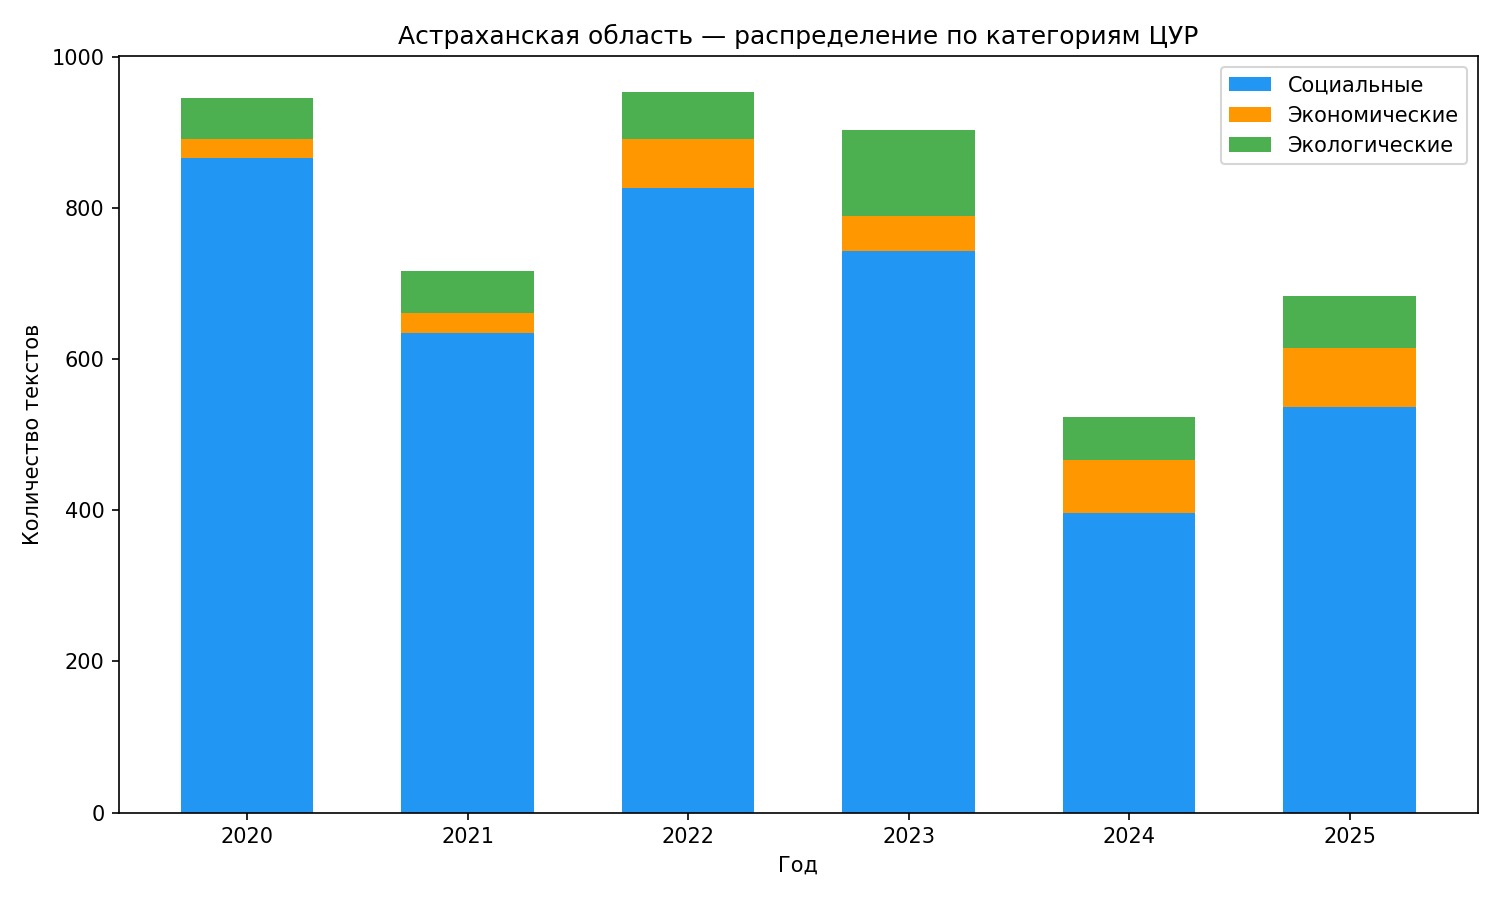
\includegraphics[width=0.68\textwidth]{fig_astrakhan_dist.png}
	\caption{Распределение текстов по категориям ЦУР, Астраханская область}
	\label{fig:astrakhan_dist}
\end{figure}

Диаграмма демонстрирует устойчивое доминирование социальной повестки в Астраханской области на протяжении всего периода наблюдения: её доля последовательно снижается с 91.6\% в 2020 году до 82.3\% в 2023 году, однако остаётся выше 80\%. Экономическая повестка представлена минимально: от 2.6\% до 6.8\%, что указывает на слабое присутствие экономической тематики в региональном новостном поле. Экологическая повестка показывает заметный рост в 2023 году (до 12.6\%), что может быть связано с конкретными региональными событиями (например, обсуждение состояния Волги или Каспийского моря).

\begin{figure}[H]
	\centering
	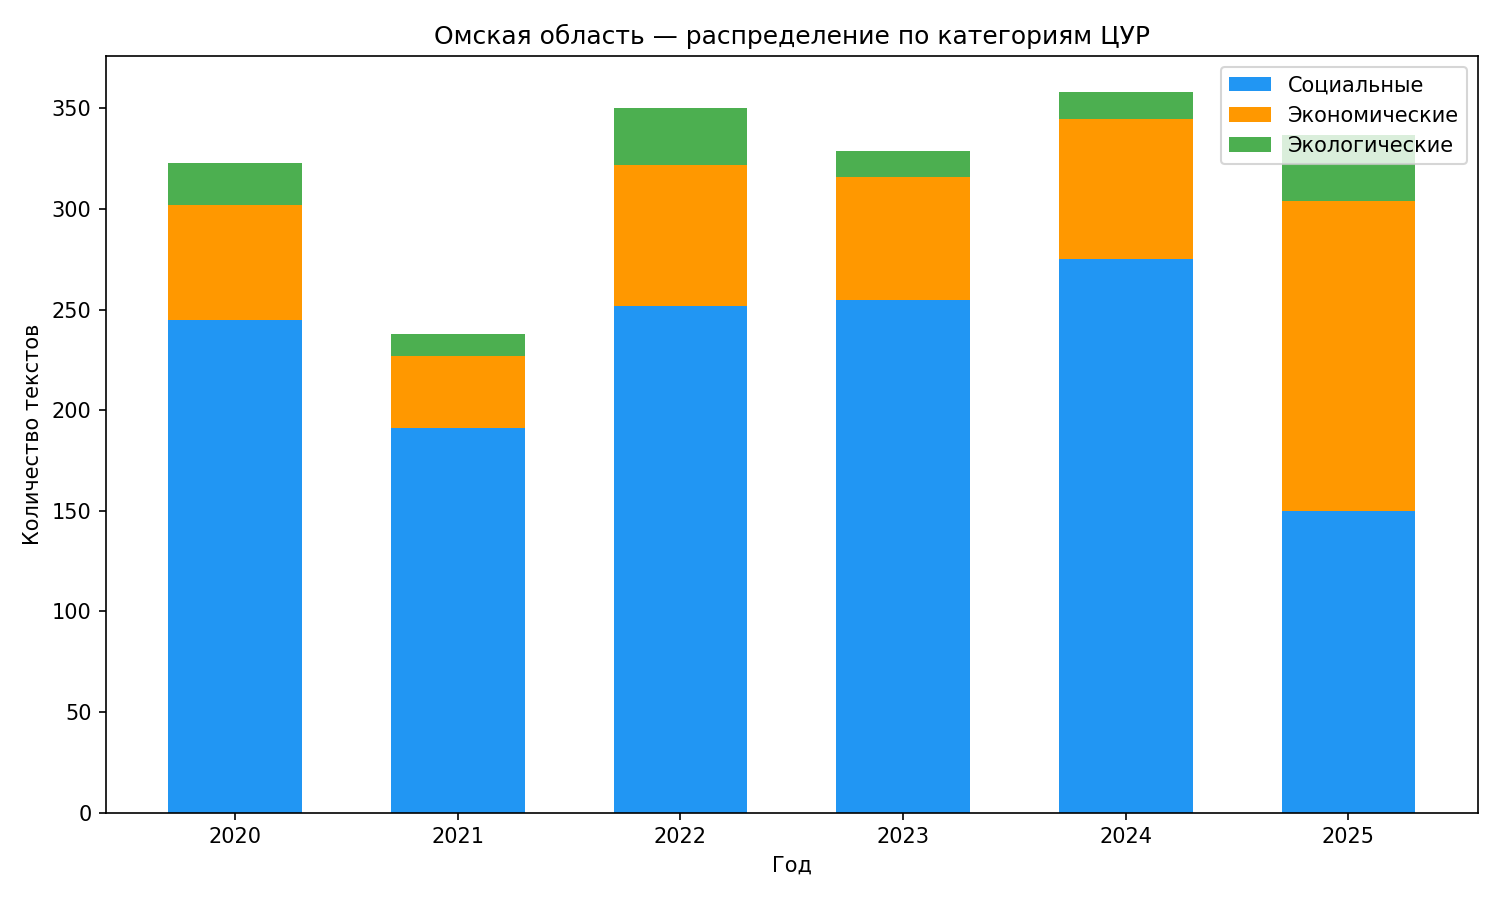
\includegraphics[width=0.68\textwidth]{fig_omsk_dist.png}
	\caption{Распределение текстов по категориям ЦУР, Омская область}
	\label{fig:omsk_dist}
\end{figure}

Диаграмма для Омской области показывает более сбалансированное распределение категорий по сравнению с Астраханской областью. Доля экономической повестки стабильно находится на уровне 15--20\%, а в 2025 году достигает пика в 45.7\%, что связано с активным обсуждением крупных инфраструктурных проектов в регионе. Социальная повестка, оставаясь доминирующей, снижается с 80\% в 2021 году до 72\% в 2022 году. Экологическая категория занимает наименьшую долю среди трёх регионов~--- 4--8\%.

\begin{figure}[H]
	\centering
	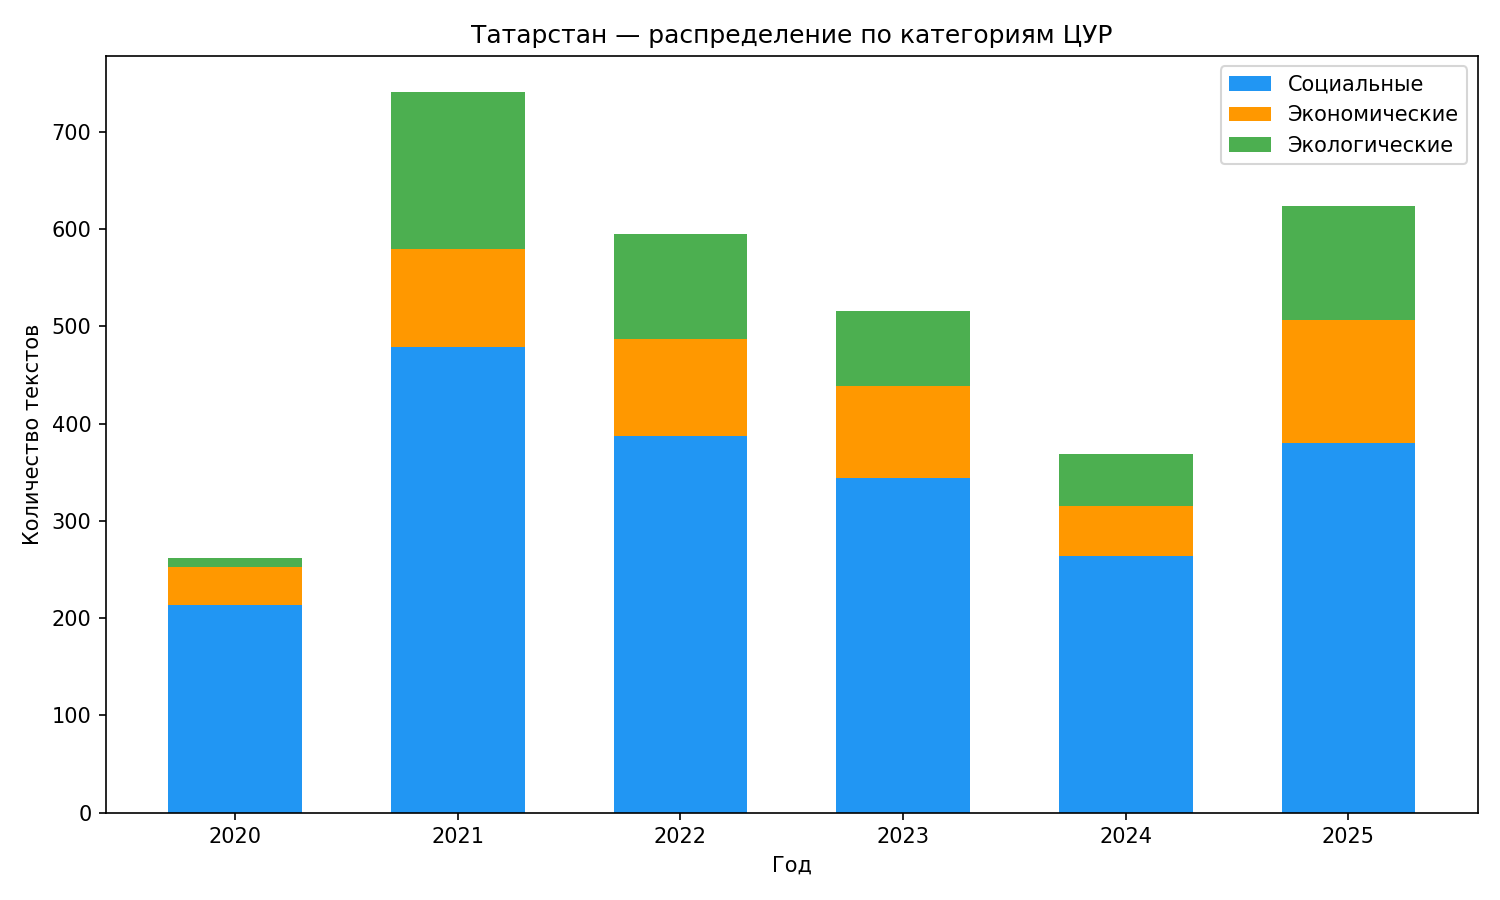
\includegraphics[width=0.68\textwidth]{fig_tatarstan_dist.png}
	\caption{Распределение текстов по категориям ЦУР, Татарстан}
	\label{fig:tatarstan_dist}
\end{figure}

Диаграмма для Татарстана демонстрирует наиболее выраженную экологическую повестку среди трёх регионов (до 21.7\% в 2021 году), а также заметный спад социальной доли с 81.3\% в 2020 году до 64.6\% в 2021 году с последующей стабилизацией на уровне 65--67\%. Экономическая повестка плавно растёт с 13.6\% в 2021 году до 18.4\% в 2023 году, что отражает повышенное внимание к вопросам промышленного развития и инноваций, характерное для региона с развитой нефтехимической и машиностроительной отраслями.

\subsubsection{Тональность по категориям ЦУР}

Результаты анализа тональности с использованием словаря КартаСловСент представлены в таблице~\ref{tab:sentiment}. Экономическая категория демонстрирует наиболее высокую долю позитивных текстов во всех трёх регионах: от 88.7\% в Татарстане до 92.7\% в Омской области. Социальная повестка характеризуется умеренно-позитивной тональностью (от 74.1\% в Татарстане до 85.1\% в Омской области). Экологическая категория, напротив, показывает наименьшую долю позитива: от 46.6\% в Татарстане до 75.2\% в Астраханской области.

\begin{table}[H]
\caption{Средняя доля позитивных текстов по категориям ЦУР и регионам (2020--2025, КартаСловСент)}
\label{tab:sentiment}
\centering\footnotesize
\begin{tabular}{|l|c|c|c|}
\hline
Регион & Социальные, \% & Экономические, \% & Экологические, \% \\
\hline
Астраханская область & 78.9 & 91.4 & 75.2 \\
Омская область       & 85.1 & 92.7 & 59.4 \\
Татарстан            & 74.1 & 88.7 & 46.6 \\
\hline
\end{tabular}
\end{table} % tab:sentiment

Результаты, полученные с использованием словаря КартаСловСент (таблица~\ref{tab:sentiment}), показывают устойчивый межкатегориальный градиент позитивности, сохраняющийся во всех трёх регионах.

На рисунке~\ref{fig:astrakhan_sent} показана динамика тональности по категориям ЦУР для Астраханской области. Экономическая повестка на протяжении всего периода сохраняет высокий уровень позитивности (в среднем выше 90\%), в то время как социальная и экологическая категории демонстрируют более выраженные колебания.

\begin{figure}[H]
	\centering
	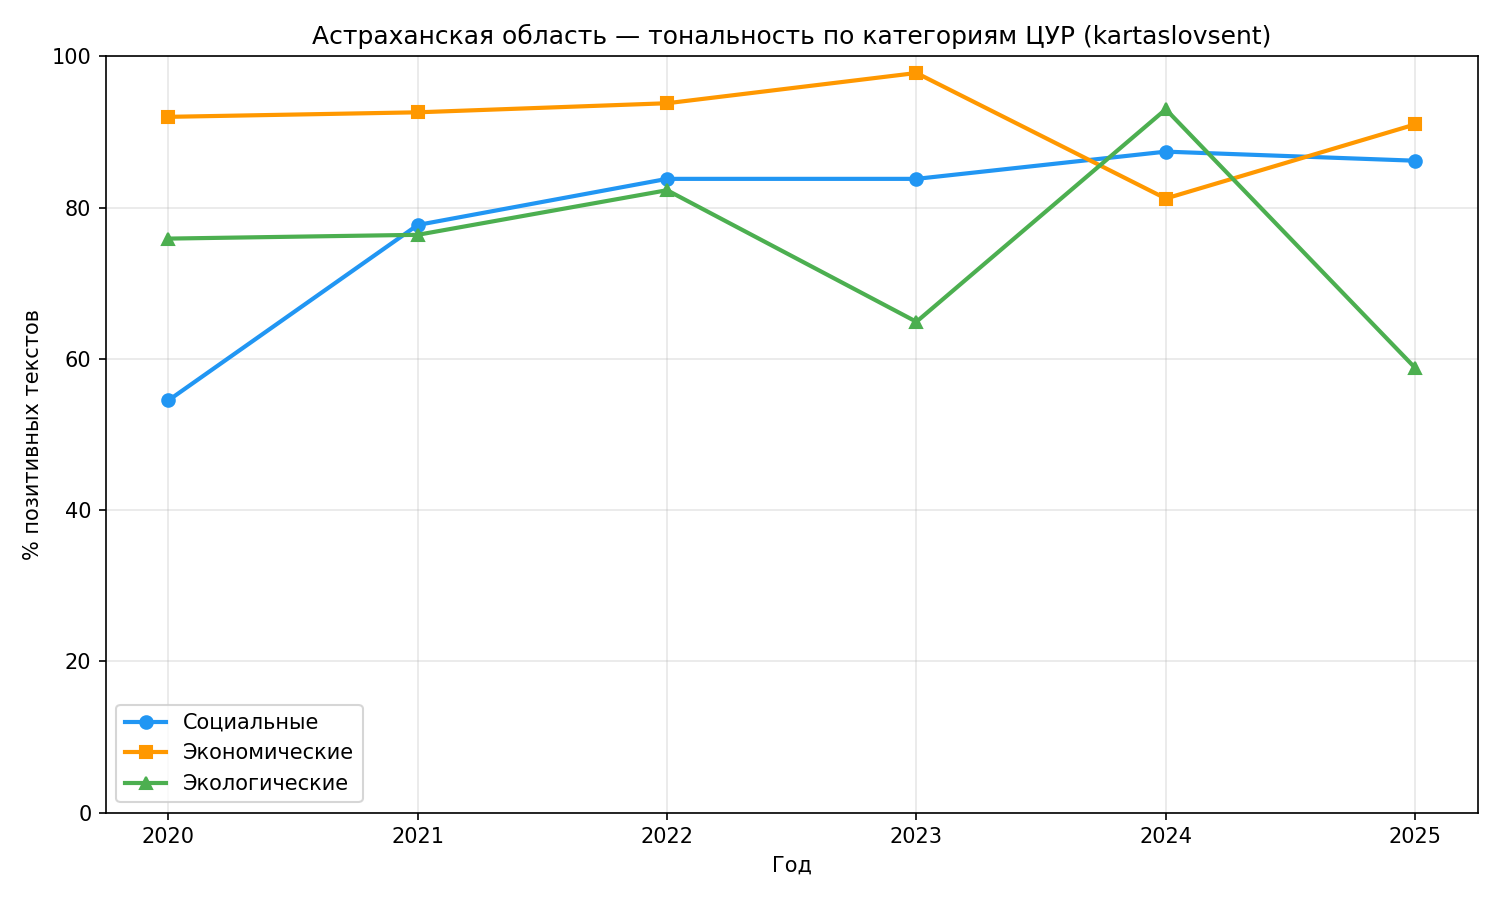
\includegraphics[width=0.68\textwidth]{fig_astrakhan_sent.png}
	\caption{Динамика тональности по категориям ЦУР, Астраханская область (КартаСловСент)}
	\label{fig:astrakhan_sent}
\end{figure}

Диаграмма отражает три важные закономерности. Во-первых, экономическая позитивность стабильно находится на уровне выше 90\% и практически не подвержена годовым колебаниям, что говорит о последовательно конструктивном характере экономических новостей. Во-вторых, социальная позитивность демонстрирует выраженный восходящий тренд с 54.5\% в 2020 году до 83.8\% в 2022--2023 годах, что может быть связано с постепенным смещением социальной повестки от кризисных тем (пандемия COVID-19) к темам развития и восстановления. В-третьих, экологическая позитивность подвержена наибольшим колебаниям (от 64.9\% до 82.3\%), что отражает нестабильный характер экологической повестки, зависящей от конкретных информационных поводов.

\subsubsection{Межрегиональное сравнение экономической повестки}

Особый интерес представляет сопоставление тональности экономической повестки между регионами (рисунок~\ref{fig:regional_comparison}). По данным словаря КартаСловСент, все три региона демонстрируют стабильно высокую позитивность экономических сообщений на уровне 85--95\%. Омская область лидирует по данному показателю (92.7\%), за ней следуют Астраханская область (91.4\%) и Татарстан (88.7\%). Высокая позитивность экономической повестки может объясняться преобладанием в новостных сообщениях материалов о развитии инфраструктуры, инвестиционных проектах и мерах государственной поддержки, которые, как правило, подаются в позитивном ключе.

\begin{figure}[H]
	\centering
	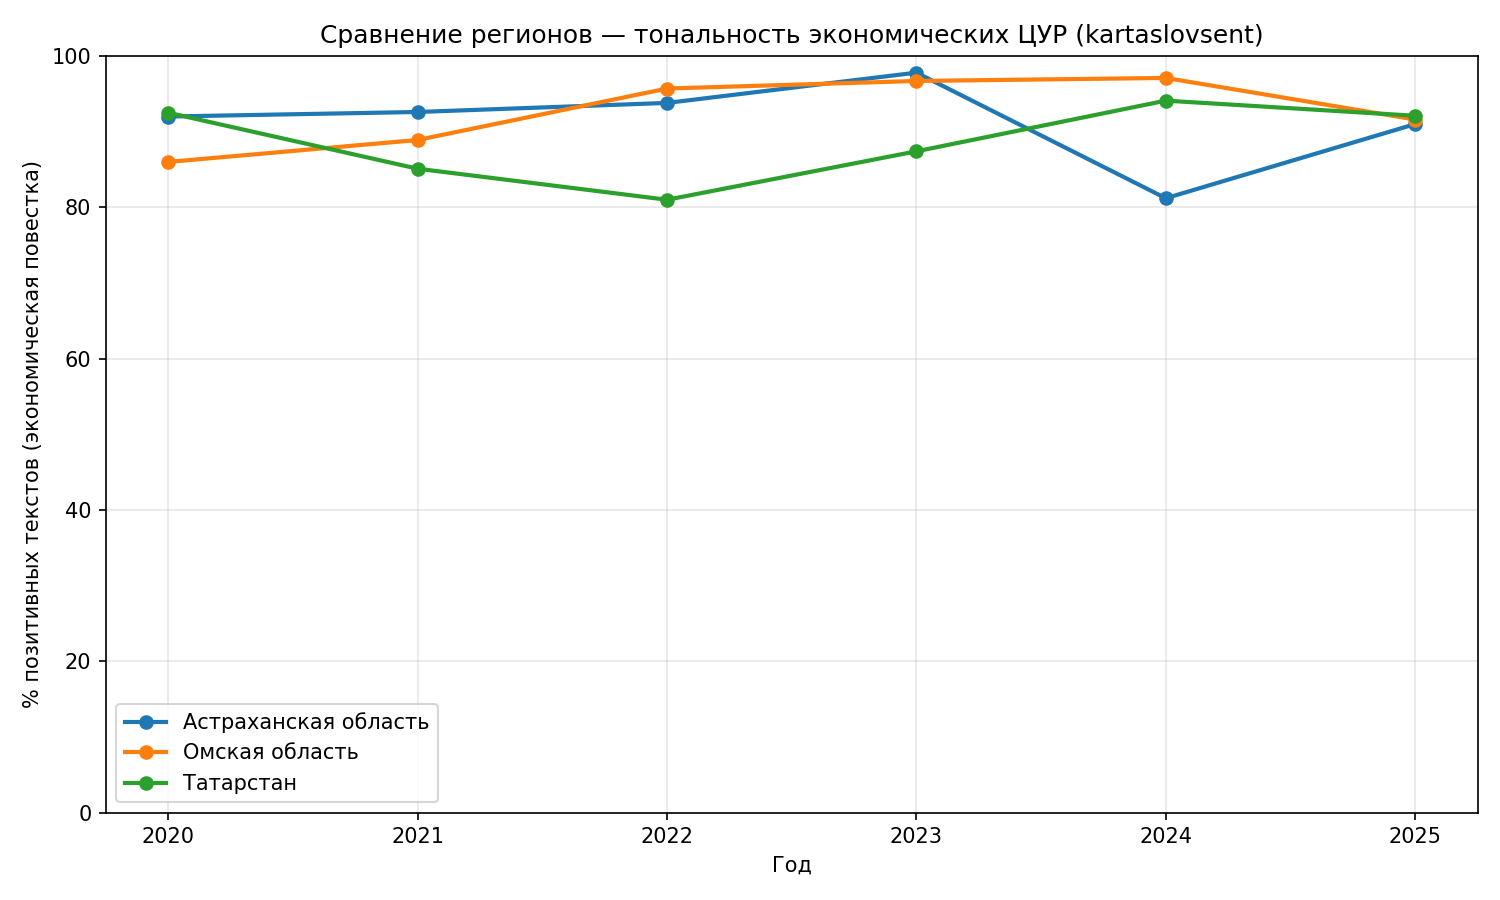
\includegraphics[width=0.68\textwidth]{fig_regional_comparison.png}
	\caption{Сравнение тональности экономической повестки по регионам (КартаСловСент)}
	\label{fig:regional_comparison}
\end{figure}

Диаграмма показывает, что, несмотря на существенные различия в уровне экономического развития регионов (ВРП на душу населения в Татарстане в 2--3 раза выше, чем в Астраханской и Омской областях), уровень позитивности экономической повестки не демонстрирует соответствующей дифференциации. Более того, наименее экономически развитая Омская область лидирует по позитивности экономических сообщений, а наиболее развитый Татарстан показывает наименьший уровень. Данное наблюдение служит эмпирическим основанием для осторожной гипотезы о том, что тональность региональной новостной повестки в социальных медиа может быть связана не только с объективным экономическим положением, но и с характером информационного освещения.

\subsubsection{Сопоставление с социально-экономическими показателями регионов}

Методологически данный этап близок к подходу~\cite{Funk2024}, где текстовая тональность сообщений, связанных с целями устойчивого развития, сопоставляется с официальными показателями прогресса по ЦУР. Выбранная логика сопоставления текстовых характеристик с внешними социально-экономическими показателями соответствует и более широкому направлению исследований, представленному, в частности, работой~\cite{Sufi2025}, где агрегированные характеристики новостного SDG-дискурса сопоставляются с макроуровневыми индикаторами стран. В обеих указанных работах объектами анализа выступают страны, тогда как в данной работе аналогичная логика применяется на региональном уровне: единицей наблюдения является пара <<регион --- год>>, а источником текстовой информации служат новостные сообщения социальной сети <<ВКонтакте>>. Объединение результатов тематической классификации, словарного анализа тональности и статистических показателей, а также расчёт корреляций и панельных регрессий выполнялись скриптом, приведённым в приложении~\ref{app:merge-code}.

По аналогии с модульной схемой анализа новостного SDG-дискурса, предложенной в работе~\cite{Sufi2025}, общую структуру данного исследования можно представить как последовательное преобразование неструктурированных текстов в агрегированные региональные индикаторы повестки, а затем в сопоставимые статистические признаки. Схематическое изображение этапов исследования приведено на рисунке~\ref{fig:pipeline}.

\begin{figure}[H]
\centering
\setlength{\fboxsep}{5pt}
\newcommand{\pipelinebox}[1]{\fbox{\parbox[c][0.9cm][c]{0.68\textwidth}{\centering\small #1}}}
\pipelinebox{Региональные сообщения VK}\\[-0.02cm]
$\downarrow$\\[-0.02cm]
\pipelinebox{SDG-классификация RuBERT}\\[-0.02cm]
$\downarrow$\\[-0.02cm]
\pipelinebox{Группировка по категориям ЦУР}\\[-0.02cm]
$\downarrow$\\[-0.02cm]
\pipelinebox{Словарная оценка тональности}\\[-0.02cm]
$\downarrow$\\[-0.02cm]
\pipelinebox{Агрегация по регионам и годам}\\[-0.02cm]
$\downarrow$\\[-0.02cm]
\pipelinebox{Объединение с показателями Росстата}\\[-0.02cm]
$\downarrow$\\[-0.02cm]
\pipelinebox{Корреляции Кендалла и FE-регрессия}\\[-0.02cm]
$\downarrow$\\[-0.02cm]
\pipelinebox{Интерпретация региональной повестки}
\caption{Этапы обработки и анализа региональной новостной повестки в контексте ЦУР}
\label{fig:pipeline}
\end{figure}

Схема показывает последовательность этапов исследования: от классификации исходных сообщений до расчёта агрегированных текстовых характеристик и их сопоставления с показателями Росстата.

Для проверки гипотезы о связи тональности новостной повестки с объективным социально-экономическим положением регионов проведено сопоставление результатов анализа с официальными статистическими данными Росстата~\cite{Rosstat2024} за 2020--2023 годы. Из ежегодного статистического сборника <<Регионы России. Социально-экономические показатели>>~\cite{Rosstat2024} для каждого региона извлечены 15 показателей, сгруппированных по трём тематическим направлениям, соответствующим категориям ЦУР:

\begin{itemize}
\item социальные: уровень безработицы, коэффициент рождаемости, смертность на 100\,тыс. населения, обеспеченность врачами и больничными койками на 10\,тыс. населения;
\item экономические: ВРП на душу населения, инвестиции в основной капитал на душу населения, среднемесячная номинальная заработная плата, оборот розничной торговли на душу населения;
\item экологические: выбросы загрязняющих веществ в атмосферу, доля уловленных и обезвреженных веществ, забор свежей воды, сброс загрязнённых сточных вод, расходы на охрану окружающей среды на душу населения.
\end{itemize}

Данные извлекались из статистических сборников за 2021, 2022, 2023, 2024 и 2025 годы (разделы 2, 3, 4, 6, 8, 9, 10, 16) с использованием скрипта, приведённого в приложении~\ref{app:extract-code}. При наличии значений в нескольких публикациях использовалась наиболее поздняя доступная редакция. Ключевые показатели за все годы приведены в таблице~\ref{tab:rosstat_raw}.

\begin{table}[H]
\caption{Ключевые социально-экономические показатели регионов по данным Росстата (2020--2023)}
\label{tab:rosstat_raw}
\centering\resizebox{\textwidth}{!}{%
\begin{tabular}{|l|c|c|c|c|c|c|}
\hline
Регион & Год & ВРП на душу, руб. & Безработица, \% & Инвестиции на душу, руб. & Средняя зарплата, руб. & Выбросы, тыс. т \\
\hline
\multirow{4}{*}{Астраханская обл.} & 2020 & 541\,099 & 7.9 & 115\,116 & 38\,885 & 112 \\
                                    & 2021 & 688\,988 & 7.8 & 115\,484 & 42\,096 & 91 \\
                                    & 2022 & 800\,576 & 7.1 & 87\,352  & 47\,780 & 104 \\
                                    & 2023 & 819\,952 & 4.4 & 89\,373  & 53\,964 & 100 \\
\hline
\multirow{4}{*}{Омская обл.}        & 2020 & 407\,371 & 8.9 & 200\,450 & 37\,828 & 147 \\
                                    & 2021 & 426\,872 & 6.5 & 191\,473 & 41\,152 & 159 \\
                                    & 2022 & 503\,176 & 5.3 & 194\,431 & 46\,952 & 165 \\
                                    & 2023 & 578\,934 & 3.6 & 208\,399 & 55\,227 & 159 \\
\hline
\multirow{4}{*}{Респ. Татарстан}    & 2020 & 658\,312 & 3.6 & 615\,593  & 39\,761 & 325 \\
                                    & 2021 & 883\,564 & 2.7 & 689\,232  & 45\,800 & 323 \\
                                    & 2022 & 1\,035\,953 & 2.3 & 888\,649  & 52\,274 & 320 \\
                                    & 2023 & 1\,145\,174 & 2.1 & 1\,180\,448 & 61\,894 & 320 \\
\hline
\end{tabular}%
}
\end{table} % tab:rosstat_raw

Для сопоставления в таблице~\ref{tab:sdg_data} приведены соответствующие характеристики новостной повестки за те же периоды: доли каждой из трёх категорий ЦУР в общем объёме сообщений и доля позитивных текстов по данным словаря КартаСловСент.

\begin{table}[H]
\caption{Характеристики новостной повестки по категориям ЦУР (2020--2023, КартаСловСент)}
\label{tab:sdg_data}
\centering\resizebox{\textwidth}{!}{%
\begin{tabular}{|l|c|c|c|c|c|c|c|}
\hline
Регион & Год & Соц., \% & Экон., \% & Экол., \% & +Соц, \% & +Экон, \% & +Экол, \% \\
\hline
\multirow{4}{*}{Астраханская обл.} & 2020 & 91.6 & 2.6  & 5.7  & 54.5 & 92.0 & 75.9 \\
                                    & 2021 & 88.5 & 3.8  & 7.7  & 77.7 & 92.6 & 76.4 \\
                                    & 2022 & 86.7 & 6.8  & 6.5  & 83.8 & 93.8 & 82.3 \\
                                    & 2023 & 82.3 & 5.1  & 12.6 & 83.8 & 97.8 & 64.9 \\
\hline
\multirow{4}{*}{Омская обл.}        & 2020 & 75.9 & 17.6 & 6.5  & 83.7 & 86.0 & 38.1 \\
                                    & 2021 & 80.3 & 15.1 & 4.6  & 84.8 & 88.9 & 18.2 \\
                                    & 2022 & 72.0 & 20.0 & 8.0  & 88.1 & 95.7 & 92.9 \\
                                    & 2023 & 77.5 & 18.5 & 4.0  & 92.5 & 96.7 & 100 \\
\hline
\multirow{4}{*}{Респ. Татарстан}    & 2020 & 81.3 & 15.3 & 3.4  & 83.6 & 92.5 & 100 \\
                                    & 2021 & 64.6 & 13.6 & 21.7 & 61.0 & 85.1 & 29.7 \\
                                    & 2022 & 65.0 & 16.8 & 18.2 & 65.1 & 81.0 & 33.3 \\
                                    & 2023 & 66.7 & 18.4 & 14.9 & 70.3 & 87.4 & 40.8 \\
\hline
\end{tabular}%
}
\end{table}

\subsubsection{Корреляционный анализ (коэффициент Кендалла)}
Сформированный набор данных имеет панельную структуру: одни и те же регионы наблюдаются в течение нескольких лет, поэтому отдельные наблюдения не являются полностью независимыми. Поскольку выборка мала ($n=12$), а распределения показателей Росстата заведомо отличаются от нормальных (три региона находятся на разных уровнях экономического развития), применение параметрического коэффициента Пирсона не вполне обосновано. В качестве основной меры связи используется непараметрический коэффициент ранговой корреляции Кендалла $\tau$, который, в отличие от коэффициента Спирмена, даёт более консервативную оценку и лучше работает при малом числе наблюдений~\cite{Funk2024}.

Коэффициент $\tau$ вычислялся с использованием реализации scipy.stats.kendalltau (вариант $\tau_b$ с поправкой на связанные ранги). Расчёт основан на попарном сравнении всех наблюдений: конкордантные пары дают положительный вклад, если порядок значений $x$ совпадает с порядком значений $y$, а дискордантные пары дают отрицательный вклад, если эти порядки противоположны. Вариант $\tau_b$ дополнительно корректирует значение коэффициента при наличии связанных рангов, то есть совпадающих значений в одном или обоих сравниваемых рядах.

Корреляционный анализ проводился попарно между двумя наборами переменных. Первый набор~--- 6 характеристик новостной повестки (доли социальной, экономической и экологической категорий в общем объёме сообщений, а также доли позитивных текстов в каждой из трёх категорий). Второй набор~--- 14 показателей Росстата, сгруппированных по трём направлениям: социальные (уровень безработицы, коэффициент рождаемости, смертность на 100\,тыс. населения, обеспеченность врачами и больничными койками на 10\,тыс. населения), экономические (ВРП на душу населения, инвестиции на душу населения, среднемесячная номинальная заработная плата, оборот розничной торговли на душу населения) и экологические (выбросы загрязняющих веществ в атмосферу, доля уловленных и обезвреженных веществ, забор свежей воды, сброс загрязнённых сточных вод, расходы на охрану окружающей среды на душу населения). Каждая пара <<характеристика повестки --- показатель Росстата>> образует набор из $n=12$ наблюдений (3 региона $\times$ 4 года, 2020--2023). Для каждого такого набора оба ряда значений преобразуются в ранги.

Ранг $R(x_i)$ величины $x_i$ в выборке объёмом $n$~--- это её порядковый номер в отсортированном по возрастанию ряду $\{x_{(1)} \le x_{(2)} \le \ldots \le x_{(n)}\}$. Например, для ряда значений ВРП на душу: 407\,371, 541\,099, 658\,312 ранги равны соответственно 1, 2, 3 (наименьшее значение получает ранг~1). При совпадении значений (связанные ранги) каждому из совпавших наблюдений присваивается среднее арифметическое их потенциальных номеров. Переход от абсолютных значений к рангам делает анализ нечувствительным к форме распределения данных и к наличию выбросов, что критически важно при малой выборке.

Коэффициент $\tau$ принимает значения от $-1$ (полная противоположность ранговых порядков) до $+1$ (полное совпадение), ноль означает отсутствие монотонной связи. Величина $p$ (p-value)~--- это вероятность получить наблюдаемое значение $|\tau|$ или ещё более экстремальное при условии, что в действительности между переменными нет никакой связи (нулевая гипотеза). Вычисление $p$ основано на асимптотической нормальности статистики Кендалла: при $n \ge 10$ стандартизованное значение $z = \tau / SE(\tau)$, где $SE(\tau)$ — стандартная ошибка $\tau$, учитывающая объём выборки и количество связанных рангов, распределено приближённо нормально. Величина $p$ вычисляется как $P(|Z| \ge |z|)$ для стандартного нормального распределения. Чем меньше $p$, тем менее вероятно, что обнаруженная корреляция случайна: $p < 0.05$ считается статистически значимым, $p < 0.01$ --- высоко значимым.

Результаты корреляционного анализа для 6 характеристик новостной повестки и 14 показателей Росстата представлены в таблице~\ref{tab:kendall}. Полная матрица содержит $6 \times 14 = 84$ пары; для компактности и содержательной интерпретации в таблицу включены только пары, для которых $|\tau| > 0.40$ (умеренная или сильная монотонная связь). Порог $0.40$ является общепринятой границей умеренной непараметрической корреляции; пары с $|\tau| \le 0.40$ при $n=12$ соответствуют слабым ассоциациям, не поддающимся содержательной интерпретации. Из 84 пар данному критерию удовлетворяют 15.

\begin{table}[H]
\caption{Коэффициент корреляции Кендалла ($\tau$) между показателями Росстата и характеристиками новостной повестки (2020--2023, $n=12$). Показаны пары с $|\tau| > 0.40$}
\label{tab:kendall}
\centering\resizebox{\textwidth}{!}{%
\begin{tabular}{|l|c|c|c|c|}
\hline
Характеристика повестки & Показатель Росстата & $\tau$ & $p$ \\
\hline
Доля соц.\ кат., \%       & Обеспеченность врачами на 10 тыс.  &  0.76 & 0.001 \\
Доля экон.\ кат., \%      & Коэффициент рождаемости           & $-0.72$ & 0.001 \\
Доля соц.\ кат., \%       & Обеспеченность койками на 10 тыс.  &  0.70 & 0.002 \\
Доля соц.\ кат., \%       & Сброс загрязнённых сточных вод     & $-0.68$ & 0.002 \\
Доля соц.\ кат., \%       & Расходы на охрану среды на душу    & $-0.64$ & 0.003 \\
Доля экон.\ кат., \%      & Расходы на охрану среды на душу    &  0.64 & 0.003 \\
Доля соц.\ кат., \%       & Выбросы в атмосферу                & $-0.59$ & 0.009 \\
Доля соц.\ кат., \%       & Инвестиции на душу                 & $-0.58$ & 0.009 \\
\hline
Доля соц.\ кат., \%       & Оборот розницы на душу             & $-0.55$ & 0.014 \\
Доля соц.\ кат., \%       & Уровень безработицы                &  0.53 & 0.016 \\
Позитивность соц., \%     & Коэффициент рождаемости           & $-0.52$ & 0.019 \\
Доля экон.\ кат., \%      & Доля уловленных загрязнителей      &  0.50 & 0.023 \\
Позитивность экон., \%    & Инвестиции на душу                 & $-0.46$ & 0.045 \\
Позитивность экон., \%    & Обеспеченность врачами на 10 тыс.  &  0.45 & 0.045 \\
Доля экол.\ кат., \%      & ВРП на душу                        &  0.44 & 0.046 \\
\hline
\end{tabular}%
}
\end{table}

Результаты корреляционного анализа указывают на то, что структурные характеристики новостной повестки (доли категорий) в рассматриваемой выборке чаще образуют более выраженные ассоциации с показателями Росстата, чем показатели тональности. Доля социальной повестки положительно коррелирует с обеспеченностью врачами ($\tau = 0.76$, $p = 0.001$) и больничными койками ($\tau = 0.70$, $p = 0.002$), а также с уровнем безработицы ($\tau = 0.53$, $p = 0.016$). Одновременно она отрицательно связана с инвестициями на душу населения ($\tau = -0.58$, $p = 0.009$), выбросами ($\tau = -0.59$, $p = 0.009$) и расходами на охрану среды ($\tau = -0.64$, $p = 0.003$). Эти результаты не следует трактовать как доказательство причинной зависимости; они скорее показывают, что в данной выборке структура региональной повестки может соотноситься с отдельными социально-экономическими характеристиками регионов.

Для показателей тональности обнаруженные ассоциации слабее и менее устойчивы. Экономическая позитивность имеет умеренную отрицательную корреляцию с инвестициями на душу населения ($\tau = -0.46$, $p = 0.045$) и не показывает значимой связи с ВРП на душу населения ($\tau = -0.03$, $p = 0.913$). Социальная позитивность отрицательно связана с коэффициентом рождаемости ($\tau = -0.52$, $p = 0.019$), однако при малом числе наблюдений такую связь следует рассматривать только как предварительное наблюдение, требующее проверки на расширенной выборке.

\subsubsection{Панельная регрессия с фиксированными эффектами}
Для проверки устойчивости корреляционных выводов и частичного учёта панельной структуры данных дополнительно проведён регрессионный анализ с фиксированными эффектами по регионам. Выбор модели с фиксированными эффектами (FE) обусловлен тремя соображениями. Во-первых, простая объединённая регрессия (pooled OLS) смешала бы межрегиональные различия с внутрирегиональной динамикой: тот факт, что Татарстан всегда богаче и при этом имеет иную структуру новостной повестки, не говорит о влиянии ВРП на тональность — он лишь отражает устойчивые различия между регионами. FE-модель, вводя индивидуальные свободные члены $\alpha_i$, отделяет эти постоянные региональные особенности от эффекта изменения переменной $x_{it}$ во времени внутри одного региона. Во-вторых, модель со случайными эффектами (RE) требует допущения о некоррелированности региональных особенностей $\alpha_i$ с регрессорами; в данном случае это допущение является сомнительным, поскольку уровень экономического развития тесно связан с принадлежностью к конкретному региону. В-третьих, при $N=3$ невозможно провести тест Хаусмана для формального выбора между FE и RE, поскольку асимптотические свойства теста не выполняются на столь малой выборке. Модель специфицирована как:
\begin{equation}
y_{it} = \alpha_i + \beta \cdot x_{it} + \varepsilon_{it},
\end{equation}
где $y_{it}$~--- характеристика новостной повестки для региона $i$ в году $t$, $x_{it}$~--- показатель Росстата, $\alpha_i$~--- фиксированный эффект региона (дамми-переменная), $\beta$~--- оцениваемый коэффициент, $\varepsilon_{it}$~--- случайная ошибка. Оценивание выполнено методом наименьших квадратов с использованием библиотеки statsmodels (класс OLS).

Статистическая значимость коэффициента $\beta$ проверяется с помощью $t$-теста. Стандартная ошибка $SE(\beta)$ вычисляется из диагональных элементов ковариационной матрицы оценок $Var(\hat{\beta}) = \hat{\sigma}^2 (X^T X)^{-1}$, где $\hat{\sigma}^2$ — остаточная дисперсия. Тестовая статистика $t = \beta / SE(\beta)$ при нулевой гипотезе $H_0: \beta = 0$ имеет распределение Стьюдента с $n - k$ степенями свободы ($k$ — число оцениваемых параметров, включая дамми-переменные регионов). Величина $p$ вычисляется как вероятность $P(|T| \ge |t|)$ для соответствующего $t$-распределения. Следует отметить, что при $N=3$ стандартные ошибки не могут быть кластеризованы по регионам, поэтому приводимые $p$-значения носят ориентировочный характер.

Результаты для восьми пар <<характеристика повестки --- показатель Росстата>> представлены в таблице~\ref{tab:panel_reg}. В связи с малым объёмом выборки ($n=12$, $T=4$, $N=3$) и, как следствие, низкой статистической мощностью, результаты следует интерпретировать как предварительные.

\begin{table}[H]
\caption{Результаты панельной регрессии с фиксированными эффектами по регионам (2020--2023, $n=12$)}
\label{tab:panel_reg}
\centering
\begin{tabular}{|l|c|c|c|}
\hline
Зависимая переменная & Независимая переменная & $\beta$ & $p$ \\
\hline
Доля экол.\ кат., \%          & ВРП на душу                 & $1.3\cdot 10^{-5}$ & 0.090 \\
Доля экон.\ кат., \%          & Инвестиции на душу          & $1.4\cdot 10^{-5}$ & 0.135 \\
Доля соц.\ кат., \%           & Уровень безработицы         & 1.35  & 0.248 \\
Позитивность экол., \%        & Выбросы в атмосферу         & 1.64  & 0.297 \\
Позитивность соц., \%         & Уровень безработицы         & $-2.02$ & 0.355 \\
Позитивность соц., \%         & ВРП на душу                 & $1.1\cdot 10^{-5}$ & 0.631 \\
Позитивность экон., \%        & Инвестиции на душу          & $-7.7\cdot 10^{-7}$ & 0.580 \\
Позитивность экон., \%        & ВРП на душу                 & $3.4\cdot 10^{-8}$ & 0.986 \\
\hline
\end{tabular}
\end{table}

Результаты панельной регрессии не противоречат наблюдениям корреляционного анализа, однако также должны интерпретироваться как предварительные. Ни одна из моделей, где зависимой переменной выступает позитивность (социальная, экономическая или экологическая), не демонстрирует статистически значимого коэффициента при соответствующем показателе Росстата ($p > 0.1$ для всех пар). Единственная пара с коэффициентом, значимым на 10-процентном уровне, связь доли экологической повестки с ВРП на душу населения ($\beta = 1.3 \cdot 10^{-5}$, $p = 0.090$), согласуется с положительной корреляцией Кендалла ($\tau = 0.44$, $p = 0.046$), но не позволяет делать строгий вывод о направлении или механизме связи.

Полученные результаты в целом согласуются с современными исследованиями медиадискурса устойчивого развития. Как показано в работе~\cite{Sufi2025}, структура новостного SDG-дискурса и его тональность могут быть связаны не только с самими целями устойчивого развития, но и с социально-экономическим и институциональным контекстом. В нашем случае это проявляется в том, что структурные характеристики региональной повестки (доли категорий) образуют более заметные ассоциации с показателями Росстата, чем показатели позитивности, которые могут в большей степени зависеть от редакционной политики и информационной повестки конкретных сообществ.

Таким образом, совокупность результатов корреляционного (Кендалл $\tau$) и регрессионного (панельная модель с фиксированными эффектами) анализа позволяет сформулировать осторожный вывод: сопоставление медиадискурса с официальной статистикой может использоваться для поиска возможных взаимосвязей между структурой региональной повестки и социально-экономическим положением регионов. При этом тональность региональной новостной повестки не следует напрямую отождествлять с объективным состоянием экономики, экологии или социальной сферы: она может отражать не только реальные процессы, но и особенности информационного отбора, редакционной подачи и текущих новостных поводов. Данный вывод согласуется с результатами исследования~\cite{Funk2024}, показавшего, что тональность текстовых SDG-нарративов в большинстве случаев не имеет прямой статистически значимой связи с официальными показателями прогресса по целям устойчивого развития.

\conclusion

В результате выполнения курсовой работы решена задача анализа тональности региональной новостной повестки в контексте целей устойчивого развития. Были собраны и обработаны 9\,765 текстовых сообщений из региональных новостных сообществ социальной сети <<ВКонтакте>> по трём субъектам Российской Федерации: Астраханской области, Омской области и Республике Татарстан за период 2020--2025 годов.

Для тематической классификации сообщений использована модель RuBERT~\cite{Kuratov2019}, дообученная на корпусе SDG-размеченных текстов~\cite{Morozov2025}. Каждое сообщение было отнесено к одной из 17 целей устойчивого развития, после чего цели были агрегированы в три укрупнённые категории: социальную, экономическую и экологическую. Это позволило перейти от анализа отдельных классов ЦУР к сопоставлению макронаправлений региональной повестки.

Проведённый анализ показал, что во всех трёх регионах доминирует социальная повестка: в среднем она составляет 74.5\% сообщений. Экономическая категория занимает меньшую долю информационного поля (15.4\%), однако характеризуется наиболее высокой позитивностью. Экологическая категория, напротив, демонстрирует наименьшую долю позитивных сообщений, особенно в Республике Татарстан.

Для оценки тональности классифицированных текстов использован словарь КартаСловСент~\cite{Kartaslovsent}, один из крупнейших русскоязычных тональных словарей (46 тыс. терминов) с дробной шкалой оценки. Выбор словаря обоснован его объёмом, детальностью разметки и актуальностью.

Выполнено сопоставление характеристик новостной повестки с 15 социально-экономическими показателями Росстата~\cite{Rosstat2024} за 2020--2023 годы. Сформированный набор данных имеет панельную структуру ($N=3$, $T=4$, $n=12$). С использованием коэффициента Кендалла и панельной регрессии с фиксированными эффектами по регионам показано, что тональность (позитивность) новостной повестки в данной выборке не обнаруживает устойчивой статистически значимой связи с ключевыми экономическими показателями, включая ВРП на душу населения. В то же время структурные характеристики повестки (распределение долей категорий) образуют более заметные ассоциации с социально-экономическими индикаторами. Эти результаты следует рассматривать не как окончательное доказательство зависимости, а как основание для дальнейшей проверки гипотезы о связи между медиадискурсом и социально-экономическим контекстом регионов.

Таким образом, проведённая работа показывает, что объединение тематической SDG-классификации, словарного анализа тональности и официальной статистики может быть перспективным способом выявления возможных взаимосвязей между медиадискурсом и положением дел в социальной, экономической и экологической сферах. Однако такие взаимосвязи требуют осторожной интерпретации: медиаповестка не является прямым отражением реальности, а формируется под влиянием новостных поводов, редакционного отбора, локального контекста и особенностей платформы.

Основным ограничением выполненного анализа является малый размер выборки: рассматриваются только три региона и четыре года, что не позволяет делать строгие выводы о характере и направлении выявленных ассоциаций. Кроме того, в работе не учитывались временные лаги между освещением события в медиапространстве и его возможным отражением в официальной статистике. Новостные сообщения могут предшествовать изменениям в экономике, экологии или социальной жизни, а могут, наоборот, реагировать на уже произошедшие процессы; при этом годовые показатели Росстата фиксируют агрегированный результат с задержкой. Поэтому связь между медиадискурсом и реальными изменениями может проявляться не синхронно, а через один или несколько последующих периодов.

Перспективными направлениями дальнейшего исследования являются расширение выборки на большее число субъектов Российской Федерации, увеличение временного горизонта, применение лаговых спецификаций, сопоставляющих медиапоказатели за год $t$ с социально-экономическими показателями последующих лет, использование аспектно-ориентированного анализа тональности и сопоставление текстовых индикаторов с более широким набором социально-экономических показателей. При таких доработках предложенный подход может стать более надёжным инструментом для анализа взаимосвязи между региональным медиадискурсом и реальными социально-экономическими процессами.

	\bibliographystyle{ugost2003}
	\bibliography{References}

\appendix

\section{Перечень ключевых слов для отбора сообщений}
\label{app:keywords}

Для отбора релевантных сообщений использовались следующие тематические группы ключевых слов:

\begin{itemize}
	\item ЦУР 1: бедность, распределение доходов, доходы населения, благосостояние, социальная безопасность;
	\item ЦУР 2: продовольственная безопасность, продовольственный суверенитет, культура питания, регенеративное сельское хозяйство, органическая еда, цена на продукты питания;
	\item ЦУР 3: психическое здоровье, общественное здравоохранение, психическое благополучие, инвалидность, санитарное просвещение, инфекционные заболевания, детская смертность, планирование семьи, неонатальная смертность, младенческая смертность, здоровье детей, дорожно-транспортные происшествия, репродуктивное здоровье, эпидемии, медицинское страхование;
	\item ЦУР 4: образование, экологическое образование, профессиональное техническое обучение, бесплатное образование, доступное образование, начальное образование, среднее образование, высшее образование;
	\item ЦУР 5: гендерное равенство;
	\item ЦУР 6: рекультивация, эффективность использования воды, истощение грунтовых вод, опустынивание, зелёная инфраструктура;
	\item ЦУР 7: возобновляемая энергия, ветровая, солнечная, геотермальная, гидроэлектрическая энергия, топливосберегающие технологии, выбросы, парниковый эффект, биотопливо;
	\item ЦУР 8: занятость, экономический рост, устойчивое развитие, заработная плата, расширение экономических прав и возможностей, малые и средние предприятия, занятость молодёжи;
	\item ЦУР 9: инфраструктура, инвестиции, интернет, промышленная диверсификация;
	\item ЦУР 10: торговля, финансовый рынок, налогообложение, социальное обеспечение, государственная программа;
	\item ЦУР 11: общественный транспорт, адаптация к изменению климата, доступное жильё, пешеходная зона, общественные пространства;
	\item ЦУР 12: природные ресурсы, переработка, промышленная экология, повторное использование, декарбонизация, пищевые отходы;
	\item ЦУР 13: климат, парниковый газ, глобальное потепление, погода, окружающая среда;
	\item ЦУР 14: защита водных ресурсов, рыбные запасы;
	\item ЦУР 15: землепользование, экологическое восстановление земель, сохранение лесов, вырубка лесов, лесовозобновление;
	\item ЦУР 16: социальная справедливость, правовая система, борьба с терроризмом.
\end{itemize}

\section{Код извлечения и агрегации показателей Росстата}
\label{app:extract-code}

В листинге приведён скрипт, использованный для извлечения показателей из статистических сборников Росстата и формирования агрегированного файла \texttt{region\_indicators.csv}.

\VerbatimInput[fontsize=\scriptsize,numbers=left,frame=single]{../../src/extract_rosstat.py}

\section{Код объединения данных и корреляционного анализа}
\label{app:merge-code}

В листинге приведён скрипт, использованный для объединения результатов SDG-классификации, словарного анализа тональности и социально-экономических показателей, а также для расчёта коэффициентов Пирсона, Спирмена и Кендалла.

\VerbatimInput[fontsize=\scriptsize,numbers=left,frame=single]{../../src/merge_and_correlate.py}
	
\end{document}
